\documentclass[a4paper,11pt]{article}
\title{Stream Ciphers: Striving for Randomness}
\date{2022\\ xth of July}
\author{Carl Schünemann\\\textit{Student No.}\and Simon Thalmaier\\\textit{Student No.}\and Larysa Bondar\\\textit{Student No.}}

%%%%%%%%%%%%%% Predefined packages
\usepackage{times,amsmath,eurosym, amssymb, color, graphicx}
\usepackage{booktabs, cellspace}
\usepackage[english]{babel} 
%%%%%%%%%%%%%% Packages: IF YOU NEED TO ADD A PACKAGE, PLEASE DO IT HERE:
\usepackage{graphicx}
\usepackage{nccmath}
\usepackage{svg}
%%%%%%%%%%%%%%%%%%%%%%%%%
%%%%%%%%%%%%%%%%%%%%%%%%%
%%%%%%%%%%%%%%%%%%%%%%%%%
%%%%%%%%%%%%%%%%%%%%%%%%%

\usepackage{csquotes}	% Steuerung der Anführungszeichen
\usepackage[
backend=bibtex,		% Sortier-Compiler
style=ieee,		% Zitationsstil
sorting=none
]{biblatex}

\addbibresource{ref.bib}




%%%%%%%%%%%%%%%%%%%%%%%%%
%%%%%%%%%%%%%%%%%%%%%%%%%
%%%%%%%%%%%%%%%%%%%%%%%%%
%%%%%%%%%%%%%%%%%%%%%%%%%
%%%%%%%%%%%%%% Useful definitions
\newcommand{\R}{\mathbb R}
\newcommand{\C}{\mathbb C}
\newcommand{\F}{\mathbb F}
\newcommand{\Z}{\mathbb Z}
\newcommand{\Q}{\mathbb Q}
\newcommand{\N}{\mathbb N}

\newcommand\veczwo[2]{\left[\begin{array}{r}#1\\#2\end{array}\right]}
\newcommand\vecdrei[3]{\left[\begin{array}{r}#1\\#2\\#3\end{array}\right]}
\newcommand\vecdreic[3]{\left[\begin{array}{c}#1\\#2\\#3\end{array}\right]}
\newcommand\vecvier[4]{\left[\begin{array}{r}#1\\#2\\#3\\#4\end{array}\right]}
\newcommand\vecsechs[6]{\left[\begin{array}{r}#1\\#2\\#3\\#4\\#5\\#6\end{array}\right]}

\newcommand\matzz[4]{\left[\begin{array}{rr}#1&#2\\#3&#4\end{array}\right]}
\newcommand\matdd[9]{\left[\begin{array}{rrr}#1&#2&#3\\#4&#5&#6\\#7&#8&#9\end{array}\right]}
\newcommand\matddc[9]{\left[\begin{array}{ccc}#1&#2&#3\\#4&#5&#6\\#7&#8&#9\end{array}\right]}
%%%%%%%%%%%%%%% 



%%%%%%%%%%%%% Page layout
\topmargin-20mm
\headheight10mm
\headsep10mm
\topskip0.1mm
\hoffset-15mm
\textwidth15.5cm
\textheight22cm
\parindent0em
%\markleft{\authors}
%\markright{\shorttitle} 
\pagenumbering{arabic}
%%%%%%%%%%%%%%%%%%


\begin{document}
\maketitle
\thispagestyle{empty}

\hrule

$\vphantom{i}$ \\[-.25cm]


%\section{Stream Ciphers}  
%$\vphantom{i}\hspace{.65cm}$  \textit{Carl Schünemann (cas0597), Larysa %Bondar (lab7449), Simon Thalmaier (sit7432) }

%$\vphantom{i}$ \\[-.25cm]

\hrule

\tableofcontents
\newpage
%%%%%%%%%%%%%%%%%%%%%%%%%%%%%%%%%%%%%%%%%%%%%%%%%%
%%%%%%%%%%%%%%%%%%%%%%%%%%%%%%%%%%%%%%%%%%%%%%%%%%
%%%%%%%%%%%%%%%%%%%%%%%%%%%%%%%%%%%%%%%%%%%%%%%%%%
%%%%%%%%%%%%%%%%%%%%%%%%%%%%%%%%%%%%%%%%%%%%%%%%%%
%%%%%%%%%%%%%%%%%%%%%%%%%%%%%%%%%%%%%%%%%%%%%%%%%%
%%%%%%%%%%%%%%%%%%%%%%%%%%%%%%%%%%%%%%%%%%%%%%%%%%
%%%%%%%%%%%%%%%%%%%%%%%%%%%%%%%%%%%%%%%%%%%%%%%%%%
%%%%%%%%%%%%%%%%%%%%%%%%%%%%%%%%%%%%%%%%%%%%%%%%%%


\section{Introduction}

Random numbers are an important component of modern cryptography. In the case of encryption, they reduce redundancies in encrypted plaintexts, resulting in more secure transmission. \cite[p. 107]{Zhang.2014} The underlying issue is the difficulty of generating random numbers. In his paper \textit{Various Techniques Used in Connection With Random Digits}, John von Neumann already warned in 1951 of this non-trivial task: “Any one who considers arithmetical methods of producing random digits is, of course, in a state of sin.” \cite[p. 36]{vonNeumann1951} A cryptographic system that addresses this challenge is stream ciphers. The generation of random numbers has a central function in this concept. Stream ciphers are used if one symbol is to be encrypted or decrypted per time unit while using minimum resources. \cite[p. 191]{Menezes.2001} \\

This paper presents efforts to approximate randomness with stream ciphers. In particular, the difficulty of this attempt will be illustrated.\\

Initially, the first chapter introduces the central idea of stream ciphers. In the second chapter, the most traditional approach for constructing stream ciphers with shift registers is discussed mathematically. Expanding on this, the third chapter  highlights the difficulties associated with this approach. Efforts to improve this idea and alternative solutions are analyzed in the fourth chapter. Finally, a recent competition is presented in the fifth chapter, aimed at determining the best of all participating stream ciphers in order to eliminate the previous difficulties.

\pagebreak


\section{The Idea of Stream Ciphers}

Stream ciphers are one of two major symmetric encryption methods. They serve a different purpose than block ciphers, the second symmetric encryption method. The primary intent is to encrypt and decrypt messages approximately synchronously between the sender and receiver of a message. To achieve this, the message is not first divided into blocks and pre-processed before it is ciphered, as is the case with block ciphers. Instead, stream ciphers encrypt or decrypt the plaintext or ciphertext directly. \cite[p. 223]{Schneier.2006} \\

A prerequisite for this is a theoretically infinite, ideally true binary random sequence. To encrypt the data, the sender combines the plaintext bitwise exclusive-or (XOR) with the random sequence. The recipient decrypts the ciphertext by also combining it bitwise exclusive-or with the same random sequence used by the sender.
\begin{figure}[h]
	\centering
	\includesvg[inkscapelatex=false, width=1\textwidth]{carl/figures/figure_1_new.svg}
	\caption{Stream cipher as a symmetric encryption method, based on \cite[p. 232]{Schneier.2006}}
	\label{fig:Figure_1}
\end{figure}
\\ This only works if both communication partners have the same random sequence. This is a characteristic of symmetric encryption. \cite[pp. 319-320]{Schmeh.2016} This problem could be trivially solved by the sender first generating a true random sequence of sufficient length and transmitting it to the recipient. However since this key sequence can also be seen as plaintext which must be transmitted securely, the situation results in a stream cipher with exactly the same problem as before.
\subsection{"True Pseudorandomness"}
The central question that arises is: How can truly random numbers be generated by means of a computer, based on a short key? \cite[p. 53]{Beutelspacher.2005} Without starting a philosophical discussion, it is necessary to define what characterizes a truly random bit sequence. \\

This can be described using an analogy to a Laplacean experiment, like the sequences of fair coin tosses: Within this sequence, the values $0$ and $1$ each occur with probability $0.5$. In addition, there is no way to derive information about the rest of the sequence from knowledge of an arbitrarily long initial piece of the sequence. To predict the next bit, an attacker must thus have no better chance of success than $0.5$. To achieve equal distribution of the bits, the experiment must be conducted theoretically for a long time. Combining a given a message $M$ with this truly random sequence XOR results in a truly random ciphertext $C$. Based on this information, a so-called \textit{perfect cipher system} is characterized by the fact that the a priori probability $P\left(M\right)$ is equal to the a posteriori probability $P({M}\mid{C})$ resulting in $P({M}\mid{C})\ = P({M})$. \cite[pp. 52-23]{Ertel.2020}

\pagebreak

The real question is in fact: Can a computer generate numbers that only look truly random? Due to the determinism of a PC, which can be represented as a finite state machine, truly random numbers can never be generated. It is only possible to generate deterministic, so-called \textit{pseudorandom numbers} (PRN). After the input of one or more initialization numbers, a \textit{pseudorandom number generator} (PRNG) generates this pseudorandom number sequence. A deterministic inner state is used for this purpose. \cite[pp. 195-196]{Ertel.2020} In the following chapters it will be shown that a stream cipher can be interpreted as a PRNG according to these criteria. As can be seen in Figure 1, a stream cipher has this inner state of the PRNG. Initially, it is filled by the short key that both communication partners possess. A stream cipher uses the key to generate and output the pseudorandom \textit{keystream} or \textit{running-key} bitwise or bytewise. \cite[p. 233]{Schneier.2006} \\

\begin{figure}[h]
	\centering
	\includesvg[inkscapelatex=false, width=0.48\textwidth]{carl/figures/figure_2_new.svg}
	\caption{A stream cipher generates the keystream with the help of the initial key, using an inner state. Based on \cite[p. 234]{Schneier.2006}}
	\label{fig:Figure_2}
\end{figure}

Optimally, this generated bit sequence should have the same statistical properties as truly random bits. To estimate this statistical quality, a series of statistical tests exist. Pioneering for the evaluation of pseudorandom numbers were the \textit{Golomb-postulates} formulated in the 1960s by the American mathematician Solomon W. Golomb. \cite[p. 43]{Golomb.1967} In order to keep the scope of this paper concise, the focus is not on this topic.\\

Ultimately, it should not be computationally feasible for an attacker to determine the prospective  sequence. No matter how many bits of the keystream one has, the probability of guessing the next bit correctly should not be better than half.


\section{Linear Feedback Shift Registers (LFSRs)}
The underlying idea of stream ciphers is the generation of a pseudorandom bit stream. An important tool for this are so called \textit{linear feedback shift registers (LFSRs)}. These kinds of shift registers are pseudorandom bit generators. This is by no means a new theory. Solomon Golomb wrote in 1967 in his book \textit{Shift Register Sequences} that the approach to generate pseudorandom sequences using LFSRs had been researched for two decades. \cite[p. 2]{Golomb.1967} Today, this idea has been developed further, resulting in many, partially theoretical applications that use shift registers. One reason for its popularity is its mathematical interpretability which is discussed in more detail in this chapter. 

\subsection{Generating Periodic Numbers}
A \textit{register} is a logical unit that has a certain number of \textit{memory cells}, each of which stores one bit of information. A set with $k$ of these cells forms a register. In the literature, no uniform term is used for these atomic elements of a register. Synonymous terms for the memory cells are, for example, \textit{memory elements} and \textit{stages} \cite[p. 81]{Stamp.2007}, \textit{delay elements} \cite[pp. 186-187]{Lidl.1986}, \textit{tubes} \cite[p. 27]{Golomb.1967} or, more broadly, \textit{bit sequence} \cite[p. 429]{Schneier.2006} or \textit{bit vector} \cite[p. 198]{Ertel.2020}. This paper uses the term memory cell as defined by Nigel P. Smart. \cite[p. 227]{Smart.2016} \\

The crucial factor of a \textit{feedback shift register} (FSR) is the connection of the memory cells via a feedback function $R$. After each clock signal, the register in its regular configuration shifts the contents of each cell to the next. In the process, one bit is shifted out at one end of the register. At the other end, a memory cell is freed. The sequence of these shifted out bits forms the sequence generated by the FSR. The new bit in the cleared memory cell at the other end is calculated by the function $R$ depending on the other bits. The shift direction differs in literature. In Smart and Schneier, for example, the shift is to the right \cite[p. 227]{Smart.2016}\cite[p. 429]{Schneier.2006} and in Lidl and Niederreiter to the left, which is adopted in this paper. The memory cell at the end where the content is shifted out has the least significant index $0$. The cell for which a new bit is calculated per clock signal has index $k-1$. \cite[pp. 186-187]{Lidl.1986}.
\begin{figure}[h]
	\centering
	\includesvg[inkscapelatex=false, width=1\textwidth]{carl/figures/figure_3_v4.svg}
	\caption{Basic concept of an LFSR of length $k=5$. The linear XOR feedback function $R$ combines the values of the tapped memory cells $0$ and $1$. Based on \cite[p. 430]{Schneier.2006}}
	\label{fig:Figure_3}
\end{figure}

The characteristic aspect of a \textit{linear feedback shift register} (LFSR) is that the new bit $k-1$ is calculated by a linear feedback function. That means, certain memory cells calculate the new value of the freed cell with the binary addition XOR. \cite[p. 82]{Stamp.2007} These memory cells whose values are used for this calculation are called \textit{tapped} \cite[p. 227]{Smart.2016}. Analogous to LFSRs, nonlinear FSRs use feedback functions, with nonlinear elements, such as binary multiplication. This concept is introduced in chapter \ref{NLFSR}. Further details can be found in Lidl and Niederreiter, 1986, page 187. \\

In literature, LFSRs are described with different mathematical approaches. Common approaches use linear algebra, polynomial algebra and the theory of finite fields \cite[pp. 186ff.]{Lidl.1986}\cite[pp. 228ff.]{Smart.2016}. Less frequently, approaches with formal power series are chosen \cite[pp. 53ff.]{Beutelspacher.2005}\cite[pp. 201ff.]{Rueppel.1986}. In this paper, the first three approaches are investigated further. \\

\pagebreak

The sequence generated by an LFSR can be described as this relation:
\begin{equation*}
s_{n+k}=a_{k-1}s_{n+k-1}+a_{k-2}s_{n+k-2}+\ldots+a_0s_n+a \;\;\;\text{for}\; n = 0,1,\ldots
\end{equation*}

The variable $s_{n+k}$ represents the value of the newly calculated bit after $n$ clock signals, which changes state of the LFSR. The values $a_0,a_1,\ldots,a_{k-1}$ indicate the tapped memory cells. The constant $a$ will be explained later. If a memory cell $a_i$ is tapped, $a_i=1$, if not $a_i=0$. For an LFSR, $a$, $a_i$ and $s_i$ are elements of the finite field $\mathbb{F}_2$. This means they are elements of the Galois field of order $p=2$, where $p$ is a prime number. This corresponds to residue field $\mathbb{Z}/2\mathbb{Z}$. \cite[p. 48]{Lidl.1997} Initially, the LFSR of length $k$ is assigned the values $s_0,\ldots,s_{k-1}\in \mathbb{F}_2$. The generated sequence $s_0,s_1,\ldots,s_{k-1},s_k,\ldots,s_{k+n}$ is thus determined by the initial values. \cite[pp. 186-187]{Lidl.1986} \\

Figure \ref{fig:Figure_4} shows an LFSR of length $k=5$ with the initial state: $s_0=1, s_1=1, s_2=0, s_3=1$ and $s_4=1$. The memory cells $0$ and $1$ are tapped, resulting in $a_0=1$ and $a_1=1$ with the remaining $a_i=0$. After a clock signal, the binary addition $a_0s_0+a_1s_1=1\cdot1+1\cdot1=0$ generates the new bit $s_{k-1+1}=s_{4+1}=s_5$, which is inserted in the freed cell after the shift 

\begin{figure}[h]
	\centering
	\includesvg[inkscapelatex=false, width=0.9\textwidth]{carl/figures/figure_4.svg}
	\caption{Workflow of an LFSR: After a clock signal, a new bit is calculated and the values of the memory cells are shifted to the left.}
	\label{fig:Figure_4}
\end{figure}

The sequence of shifted-out bits generated by an LFSR of length $k$ is called a \textit{$k$-th-order linear recurring sequence}. A distinction is made between \textit{homogenous} $k$-th-order linear recurring sequences when $a=0$ and \textit{inhomogeneous} $k$-th-order linear recurring sequence when $a\neq0$. The last case corresponds to the addition of a constant value in $\mathbb{F}_2$ to the equation above. \cite[p. 186]{Lidl.1986} Since LFSRs are usually constructed to produce homogenous $k$-th-order linear recurring sequences, the case $a\neq0$ is not considered further here. \\

As the name suggests, it is characteristic of $k$-th-order linear recurring sequences that they will repeat. A sequence is said to be \textit{periodic} if it will repeat after $r\in\mathbb{N}$ generated bits, such that $s_{n+r}=s_n$ for all $n\in\mathbb{N}_0$, where $r$ denotes the period of the sequence. This periodic behavior can possibly occur after $n_0\in\mathbb{N}_0$ non-periodic bits, such that: $s_{n+r}=s_n$ for all $n\ge{n_{0}}$. In this case the sequence is referred to as \textit{ultimately periodic} and $n_0$ as \textit{preperiod}. Any $k$-th-order linear recurring sequence with elements of $\mathbb{F}_2$ generated by an LFSR of length $k$ is ultimately periodic. The period $r$ takes at most the value $r\le2^{k}-1$. This can be explained since a register of length $k$ can only hold $2^{k}-1$ non-zero states. To avoid the trivial zero period, an LFSR of length $k$ must not be initialized with the zero sequence $s_0=s_1=\ldots=s_{k-1}=0$. \cite[p. 189]{Lidl.1986} \\

Figure \ref{fig:Figure_5} shows how the LFSR of length $k=5$ from the previous example generates a sequence of period $r=3$. The register returns to the initial state after $3$ clock signals. The preperiod is $n_0=0$.

\begin{figure}[h]
	\centering
	\includesvg[inkscapelatex=false, width=0.75\textwidth]{carl/figures/figure_5.svg}
	\caption{Periodic behavior of an LFSR. Once the state of an LFSR occurs a second time, the generated sequence will repeat.}
	\label{fig:Figure_5}
\end{figure}

Depending on the chosen values for $s_0,\ldots,s_{k-1}\in \mathbb{F}_2$ a different sequence with a possibly different period can be obtained. This can be illustrated by the following example: For each period, a state diagram is plotted. State $i$ in the diagram corresponds to an inner state of the LFSR in decimal notation. This state is formed by the contents of the memory cells $0$ to $k-1$ at a point in time. A state transition is created by applying the feedback function $R$. This representation is adapted from Nigel P. Smart in \cite[pp. 230]{Smart.2016}. Figure \ref{fig:Figure_6} shows all $32$ states of the LFSR of length $k=5$ from the previous two examples. 

\begin{figure}[h]
	\centering
	\includesvg[inkscapelatex=false, width=0.87\textwidth]{carl/figures/figure_6_new.svg}
	\caption{Representation of different periods of an LFSR as state machine diagrams. Based on \cite[pp. 230-232]{Smart.2016}}
	\label{fig:Figure_6}
\end{figure} 

\pagebreak

\subsection{m-sequences with Primitive Polynomials}
Consequently, the ultimate goal is to generate a pseudorandom number with the largest possible period. One option of trial and error is to select other tapped memory cells and check if the period has improved. Additionally, the choice of initialization values is limited, since different values for the same register may produce sequences with different periods. Such an effort is unfavorable for a symmetric encryption system. The most favorable situation would be to always generate a sequence with the largest possible period for an LFSR, regardless of the initialization vector chosen.\\

To achieve this situation, a second way must be presented to describe homogeneous $k$-th-order linear recurring sequences: An LFSR of length $k$ can be represented as the following regular $k\times{k}$ matrix $A$ over $\mathbb{F}_2$: the matrix elements $e$ in the diagonal below the main diagonal are assigned $1$: $e_{2,1},e_{3,2},\ldots,e_{k,k-1}=1$. The values of the tapped memory cells $a_i$ as defined above, are written in the $k$-th column in ascending order by index. \cite[p. 191]{Lidl.1986} For consistency, the notation of the matrix was adopted from Lidl and Niederreiter. Nigel P. Smart transposes the matrix \cite[p. 218]{Smart.2016}. As a result, the matrix $A\in \mathbb{F}_2^{k\times{k}}$ has this form:

\begin{equation*}
	\begin{pmatrix}
		0&0&0&\ldots&0&a_0\\
		1&0&0&\ldots&0&a_1\\
		0&1&0&\ldots&0&a_2\\
		\vdots&\vdots&\vdots&\ &\vdots&\vdots\\
		0&0&0&\ldots&1&a_{k-1}\\
	\end{pmatrix}
	\;\;\;\text{if }k=1,A\;\text{is the}\; 1 \times 1\;\text{matrix}\; (a_0)
\end{equation*}

The crucial point is the examination of the characteristic polynomial $f(x)$ of the matrix: 

\begin{equation*}
	f(x)=det(xI-A)=x^k-a_{k-1}x^{k-1}-a_{k-2}x^{k-2}-\ldots-a_0\in\mathbb{F}_2[x]
\end{equation*}

In the case of an LFSR, this polynomial is an element of the polynomial ring
$\mathbb{F}_2[x]$ over the finite field $\mathbb{F}_2$. Therefore, the coefficients of the polynomial – meaning the tapped memory cells – are elements of the finite field $\mathbb{F}_2$ \cite[pp. 18-19]{Lidl.1997}. Therefore, the signs of the coefficients before the indeterminant $x$ can be reversed:

\begin{equation*}
	f(x)=x^k+a_{k-1}x^{k-1}+a_{k-2}x^{k-2}+\ldots+a_0\in \mathbb{F}_2[x]
\end{equation*}

Only with the use of this characteristic polynomial it is possible to construct an LFSR which generates so-called \textit{maximal period sequences} with elements of $\mathbb{F}_2$. This refers to a sequence with the largest possible period and without preperiod, generated by an LFSR for any initial values except $0$. These sequences are also denoted as \textit{m-sequences}. Such sequences are generated by an LFSR of length $k$ if the characteristic polynomial of the matrix $A$ is a so-called \textit{primitive polynomial} in $\mathbb{F}_2[x]$. The period for all initial values except the zero initialization is $2^{k}-1$. \cite[p. 201]{Lidl.1986} \\

In the literature it is difficult to find a coherent and uniform explanation to primitive polynomials. For this paper the approach of Lidl and Niederreiter via finite fields was chosen.\\

Defining a primitive polynomial starts with the polynomial $f$ in $\mathbb{F}_2[x]$ of degree $m\ge1$. For an element $\alpha$ in $\mathbb{F}_{2^m}$ it must hold that $f(\alpha)=0$ is satisfied, whereby $\alpha$ is called the \textit{root} of $f$. The finite field $\mathbb{F}_{2^m}$ consists of the elements of $\mathbb{F}_2[x]$ modulus the polynomial $f$, resulting in $\mathbb{F}_{2^m}=\mathbb{F}_2[x]/f(x)$. \cite[p. 11]{Smart.2016} At the same time, $f$ must be the so-called \textit{minimal polynomial} of $\alpha$: Besides the property $f(\alpha)=0$, it must not be possible to factor it into further polynomials in $\mathbb{F}_2[x]$ of degree greater $0$. This property is comparable to that of a prime number. Moreover, if there is a polynomial $g$ in $\mathbb{F}_2[x]$ for which also holds $g(\alpha)=0$, then $g$ must divide the minimal polynomial $f$. The crucial characteristic of a minimal polynomial $f$ is that it is the polynomial of minimal degree with $f(\alpha)=0$, where the leading coefficient must be $1$. For this polynomial $f$ to be finally a primitive polynomial, it must hold that $\alpha$ generates the multiplicative group $\mathbb{F}_{2^m}^\times$. This group is equal to $\mathbb{F}_{2^m}$ without the $0$. Thus $\langle\alpha\rangle=\mathbb{F}_{2^m}^\times$ must hold. \cite[pp. 23, 31, 89]{Lidl.1997} \\

Just as it is difficult to test whether a number is prime, it is complex to find out whether a polynomial is primitive. \cite[p. 431]{Schneier.2006} Therefore, in the following example, we will only show that a given primitive polynomial satisfies the properties above: \\

Given is the primitive polynomial $f(x)=x^4+x^1+1$ in $\mathbb{F}_2[x]$ of degree $m=4$. For $\alpha \in \mathbb{F}_{2^4}$ holds $f(\alpha)=0$. This is how the finite field $\mathbb{F}_{2^4}=\mathbb{F}_2[x]/(x^4+x^1+1)$ is composed:
\vspace{-0.5 cm}
\begin{center}
	\begin{tabular}{l l l l l l l l}
		   	$0$	& 	$1$ \\
			$\alpha$	&	$\alpha+1$ \\
			$\alpha^2$	&	$\alpha^2+1$	&	$\alpha^2+\alpha$	&	$\alpha^2+\alpha+1$ \\ 
			$\alpha^3$	&	$\alpha^3+1$	&	$\alpha^3+\alpha$	&	$\alpha^3+\alpha+1$	&	$\alpha^3+\alpha^2$ 	&	$\alpha^3+\alpha^2+1$	&
			$\alpha^3+\alpha^2+\alpha$	& $\alpha^3+\alpha^2+\alpha+1$
	\end{tabular}
\end{center}
It can be assumed that the polynomial $f$ is a minimal polynomial. Now it will be shown that $\langle\alpha\rangle=\mathbb{F}_{2^m}^\times$, meaning that $\alpha$ generates the multiplicative group $\mathbb{F}_{2^m}^\times$.
\begin{center}
	\begin{tabular}{c c}
		$\begin{aligned}[t] % placement: default is "center", options are "top" and "bottom"
			\alpha^1 &= \alpha\\
			\alpha^2 &= \alpha^2 \\
			\alpha^3 &= \alpha^3 \\
			\alpha^4 &= \alpha + 1 \\
			\alpha^5 &= \alpha(\alpha^4)=\alpha(\alpha+1) \\
					 &= \alpha^2 + \alpha \\
			\alpha^6 &= \alpha^2\alpha^4 = \alpha^2(\alpha+1) \\
					 &= \alpha^3 + \alpha^2 \\
			\alpha^7 &= \alpha^3\alpha^4 = \alpha^3(\alpha+1) = \alpha^4\alpha^3 \\
					 &= \alpha^3+\alpha+1 \\
			\alpha^8 &= \alpha^4\alpha^4 = (\alpha + 1)(\alpha+1) \;\;\;\;\;\;\;\;\;\;\;\;\;\;\;\;\;\;\; \\
					 &= \alpha^2 + 2\alpha + 1 \\
					 &= \alpha^2 + 1 \\
			\alpha^9 &= \alpha^5\alpha^4 = (\alpha^2+\alpha)(\alpha+1) \\
					 &= \alpha^3 + \alpha^2 + \alpha^2 + \alpha \\
					 &= \alpha^3 + \alpha \\
			\alpha^{10}&= \alpha^5\alpha^5 = (\alpha^2+\alpha)(\alpha^2+\alpha) \\
					 &= \alpha^4 + 2\alpha + \alpha^2 \\
					 &= \alpha^2 + \alpha + 1 \\
		\end{aligned}$
		& 
		$\begin{aligned}[t] % placement: default is "center", options are "top" and "bottom"
			\alpha^{11} &= \alpha^5\alpha^6 = (\alpha^2+\alpha) (\alpha^2 + \alpha) \\
						&= \alpha^5+\alpha^4+\alpha^4+\alpha^3 \\
						&= \alpha^3+\alpha^2+\alpha \\
			\alpha^{12} &= \alpha^6\alpha^6 = (\alpha^3+\alpha^2)(\alpha^3+\alpha^2) \\
						&= \alpha^6 + 2\alpha^5 + \alpha^4 \\
						&= \alpha^3+\alpha^2+\alpha+1 \\
			\alpha^{13} &= \alpha^6\alpha^7 = (\alpha^3+\alpha^2)(\alpha^3+\alpha+1) \\
						&= \alpha^6 + \alpha ^4 + \alpha^3 + \alpha^5 + \alpha^3 + \alpha^2 \\
						&= \alpha^3 + \alpha^2 + \alpha + 1 + \alpha^2 + \alpha + \alpha^2 \\
						&= \alpha^3 + \alpha^2 + 1 \\
			\alpha^{14} &= \alpha^7\alpha^7 = (\alpha^3 + \alpha + 1)(\alpha^3 + \alpha + 1) \\
						&= \alpha^6 + \alpha^2 + 1 + 2\alpha^3\alpha + 2\alpha^3 + 2\alpha \\
						&= \alpha^3 + \alpha^2 + \alpha^2 + 1 \\
						&= \alpha^3 + 1 \\
			\alpha^{15} &= \alpha^8\alpha^7 = (\alpha^2 + 1)(\alpha^3 + \alpha + 1) \\
						&= \alpha^5 + \alpha^3 + \alpha^2 + \alpha^3 + \alpha + 1 \\
						&= \alpha^2 + \alpha + \alpha^2 + \alpha + 1\\
						&= 1
		\end{aligned}$
	\end{tabular}
\end{center}

\pagebreak

Consequently, $f(x)=x^4+x^1+1$ satisfies the properties of a primitive polynomial. The corresponding LFSR shown in figure \ref{fig:Figure_7} can be obtained with the help of the definition of the characteristic polynomial introduced previously: $f(x)=x^k+a_{k-1}x^{k-1}+a_{k-2}x^{k-2}+\ldots+a_0\in \mathbb{F}_2[x]$ \\

\begin{figure}[h]
	\centering
	\includesvg[inkscapelatex=false, width=0.9\textwidth]{carl/figures/figure_7_new.svg}
	\caption{Structure of the LFSR which corresponds to the primitive polynomial $f(x)=x^4+x^1+1$,  based on \cite[p. 430]{Schneier.2006}}
	\label{fig:Figure_7}
\end{figure} 

The corresponding state machine diagram for this LFSR of length $k=4$ is shown in figure \ref{fig:Figure_8}. As can be seen, apart from the trivial zero period, only one period with maximum length $2^{k}-1=2^{4}-1=15$ exists. Thus, this LFSR, of which the characteristic polynomial is primitive, produces an m-sequence. 

\begin{figure}[h]
	\centering
	\includesvg[inkscapelatex=false, width=0.51\textwidth]{carl/figures/figure_8_new.svg}
	\caption{State machine diagram of the largest possible period of an LFSR whose characteristic polynomial is primitive. Based on  \cite[pp. 230-232]{Smart.2016}}
	\label{fig:Figure_8}
\end{figure}

Proof that such a primitive polynomial indeed generates an m-sequence is difficult to find in the literature. In many cases there are references to other authors or textbooks, without going into more detail or naming them. See, for example \cite[p. 229]{Smart.2016}. I wanted to have found a coherent explanation in the literature to the question: \textit{"Why do primitive polynomials in $\,\mathbb{F}_2[x]$ of degree $k$ generate sequences with maximum period $2^{k}-1$?"} For this paper, the example shown above should be sufficient. \\

In addition to having the longest possible period, m-sequences satisfy Solomon Golomb's randomness criteria mentioned initially \cite[p. 2847]{Gong.2018}. Thus, m-sequences are statistically secure pseudorandom numbers. However, the fact that a statistically secure pseudorandom number, such as the m-sequence, does not necessarily equal a cryptographically secure number will be discussed in the next chapter.

\pagebreak



\newcommand{\comment}[1]{} 
\newcommand{\note}[1]{{\color{red} #1}}
\newcommand{\revisit}[1]{{#1}}
\newcommand*{\logeq}{\ratio\Leftrightarrow}
\newcommand*{\logright}{\ratio\Rightarrow}

\subsection{Weaknesses of LFSRs}

\subsubsection{Linear complexity of a pseudorandom number}

\subsubsection{Cracking LFSR: The Berlekamp-Massey algorithm}


\subsection{Combining multiple LFSRs} 



	\section{Strongest Stream Ciphers - eSTREAM Contest}
	
	eSTREAM was a crypto-contest held from 2004 till 2008 and aimed at discovering especially well-designed stream ciphers. eSTREAM came about due to another contest, NESSIE, which had no winners in the "Stream Ciphers" category because all of the ciphers had considerable vulnerabilities. Then, at the RSA Data Security Conference, it was argued whether stream ciphers can be considered obsolete if the Advanced Encryption Standard (AES) offers good solutions most of the time. However, there had been arguments that supported stream ciphers describing their advantages over block ciphers \cite{robshaw2008estream}:
	\begin{itemize}
		\setlength\itemsep{0.1em}
		\item Exceptionally high throughput in software.
		\item Exceptionaly low resource consumption in hardware.
	\end{itemize}
	To prove this, the European Network of Excellence for Cryptology (ECRYPT) launched the eStream project. It had three phases and featured different stream cipher designs in two Profiles \cite{robshaw2008estream}:
	\begin{itemize}
		\item[] Profile 1: Stream ciphers for software applications with high throughput.
		\item[] Profile 1A: Ciphers that satisfy Profile 1 with an associated authentification method.
		\item[] Profile 2: Stream ciphers for hardware applications with highly restricted resources (limited storage, gate count, or power consumption).
		\item[] Profile 2A: Ciphers that satisfy Profile 2 with an associated authentification method.
	\end{itemize}
	
	The following table pictures the initial requirements for the candidates:
	\begin{table}[h!]
		\centering
		\begin{tabular}{| c c c c|} 
			\hline
			& key length (bits) & IV length (bits) & tag length (bits) \\ [0.5ex] 
			\hline
			Profile 1 & 128 & 64 and 128 & - \\ 
			Profile 1A & 128 & 64 and 128 & 32, 64, 96 or 128 \\
			Profile 2 & 80 & 32 and 64 & - \\
			Profile 2A & 80 & 32 and 64 & 32 or 64 \\[1ex] 
			\hline
		\end{tabular}
		\label{table:Initial requirements for the candidates}
	\end{table}
	
	\textbf{Software-optimized ciphers} should significantly outperform the AES when used in a suitable stream cipher mode to justify stream cipher usage. It is important to point out that the contestants did not try to develop ciphers that were good at everything. The main focus was laid on raw encryption speed by large amounts of data after a single initialization. The security level was standard 128 bit, which matched contemporary applications very well.
	To evaluate all the contestants fairly, a special testing framework was introduced \cite{canniere2008estream}. It consisted of a collection of shell scripts and C-code and tested three aspects of every submitted cipher:
	\begin{enumerate}
		\item \emph{API compliance} checked if all the API requirements, like necessary interface, and key sizes are correct, if calls to the same function with the same parameters produce the same results or whether the encryption functions produce the same encrypted text from the same plaintext. 
		\item \emph{Correctness} of the code was verified by generating and comparing test vectors.
		\item \emph{Performance} was tested through the following criteria:
		\begin{itemize}
			\item \emph{Encryption rate} for long streams.
			\item\emph{Packet encryption} tested at which packet length a stream cipher would take the lead from a block cipher.
			\item \emph{Agility} tested the time spent switching from one session to another when encrypting many streams in parallel on one processor.
			\item \emph{Key and Initial Vector (IV) setup efficiency}.
		\end{itemize}
	\end{enumerate}
	
	\textbf{Hardware-optimized ciphers} should be significantly smaller and faster  than AES in a restricted environment in at least one significant aspect \cite{good2008asic}. These ciphers would be useful in, for example, sensor networks that are especially constrained in the number of logic gates or power. For this reason, the security level was chosen to be 80 bits.
	
	Like with any stream ciphers, an initialization vector (IV) and a secret key had to be used. For the 1A and 2A profiles, an authentification tag was also required.\\
	There were several evaluation criteria for each phase:
	\begin{itemize}
		\setlength\itemsep{0.1em}
		\item Security.
		\item Performance when compared to the AES in an appropriate mode.
		\item Performance, when compared to other submissions.
		\item Justification and supporting analysis simplicity and flexibility.
		\item Completeness and clarity of submission.
	\end{itemize}
	
	To go to the next phase a submission had to be notably better than AES.\\
	eSTREAM lasted four years and in 2008 a voting at SASC 2008 took place, where the finalists of the eSTREAM were evaluated on a scale from -5 to +5 and then the average was calculated. It is important to point out that this evaluation was not held by eSTREAM and should only be used for illustration. The following table demonstrates the results of the voting:
	\begin{table}[h!]
		\centering
		\begin{tabular}{|c c |c| c c|} 
			\hline 
			Rabbit & 2.80 & & Trivium & 4.35\\ 
			Salsa20 & 2.80 & & Grain v1 & 3.50\\
			SOSEMANUK & 1.20 & & MICKEY v2& 0.17\\
			HC-128 & 0.60 & & & \\[1ex]
			\hline
		\end{tabular}
		\label{table:eStream portfolio with SASC2008 evaluation}
	\end{table}
	
	This table also shows that the opinions about the hardware-optimized ciphers were more unified than the ones about the software-optimized ones.
	The ciphers that made it into the eStream portfolio can be divided into several categories \cite{jiao2020stream}:
	\begin{description}
		\item [ARX-based] (Addition/Rotation/XOR) are ciphers that only use module addition, interword rotation, and XOR to achieve required security strength. These operations are fast and easy to implement in software as well as they are immune to timing attacks because they run in constant time \cite{jiao2020stream}.
		Among the ciphers that made it into the eStream portfolio Rabbit and Salsa20 belong to ARX-based stream ciphers.
		\begin{figure}[h]
			
			\begin{subfigure}{0.5\textwidth}
				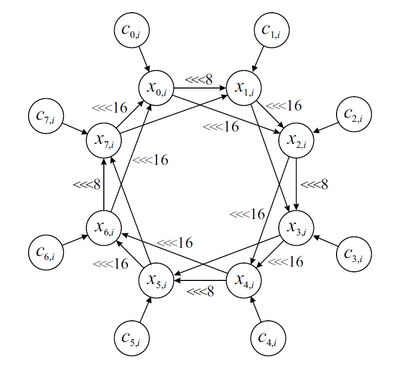
\includegraphics[width=1\textwidth]{img/rabbit.png} 
				\caption{Internal structure of the Rabbit cipher}
				\label{fig:rabbit}
			\end{subfigure}
			\begin{subfigure}{0.5\textwidth}
				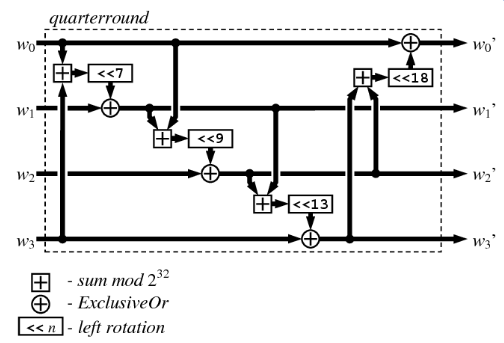
\includegraphics[width=1\textwidth]{img/salsa20.png} 
				\caption{Internal structure of the Salsa20/r ciphe}
				\label{fig:salsa20}
			\end{subfigure}
			
			\caption{ARX-based eStream finalists}
			\label{fig:arx}
		\end{figure}
		
		\emph{Rabbit} is a software-efficient, synchronous stream cipher that uses a 128-bit key and a 64-bit IV. A set of eight state registers, each 32-bit long and eight 32-bit counters are used to provide encryption based on ARX operations. Testing during the eSTREAM process confirmed that the Rabbit cipher was one of the most efficient software-oriented stream ciphers submitted \cite{boesgaard2008rabbit}.\\
		\emph{Salsa20/r} is a software-oriented cipher that supports keys of 128 bits and 256 bits. During its operation, the key, a 64-bit nonce (unique message number), a 64-bit counter, and four 32-bit constants are mapped to the 512-bit initial state. After r iterations of the Salsa20/r round function, the updated state is used as a 512-bit keystream output. Due to its implementation Salsa20 resembles a block cipher \cite{bernstein2008salsa20}.
		Although many attacks on Rabbit and Salsa20 have been proposed, as of 2015, none of them have been more successful than brute force attacks. 
		\item [NLFSR-based] stream ciphers take NLFSR as the basic components. It uses both the nonlinear feedback and the nonlinear output to provide good sequence properties and security \cite{jiao2020stream}. 
		Among the eStream finalists, Trivium and Grain v1 belong to NLFSR-based ciphers.
		
		\begin{figure}[h]
			
			\begin{subfigure}{0.5\textwidth}
				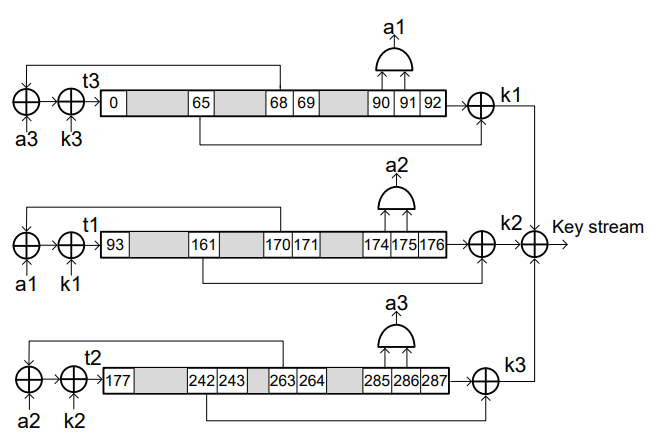
\includegraphics[width=1\textwidth]{img/trivium.png} 
				\caption{Internal structure of the Trivium cipher}
				\label{fig:trivium}
			\end{subfigure}
			\begin{subfigure}{0.5\textwidth}
				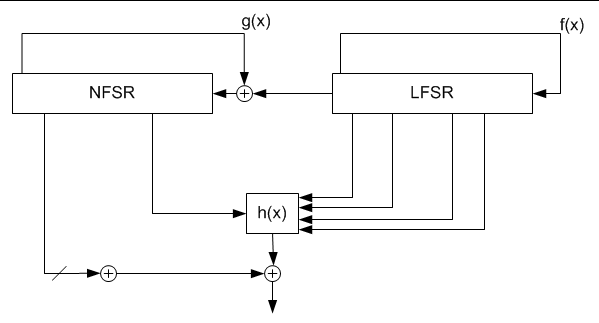
\includegraphics[width=1\textwidth]{img/grainv1.png} 
				\caption{Internal structure of the Grain v1 cipher}
				\label{fig:grainv1}
			\end{subfigure}
			
			\caption{NLFSR-based eStream finalists}
			\label{fig:NLFSR}
			
		\end{figure}
		
		\emph{Trivium} is a hardware-oriented stream cipher the main advantage of which is its simple design. It consists of three interconnected NLFSRs with feedback functions and linear or quadratic filter functions. It takes an 80-bit key and an 80-bit IV, and generates up to 264 keystream bits. It is important to note that Trivium was designed as an exercise, to explore how far a stream cipher can be simplified without sacrificing its security, speed or flexibility and still outperform AES \cite{canniere2008trivium}.\\
		\emph{Grain v1} combines the LFSR with the NLFSR, where LFSR provides good statistical characteristics and NLFSR adds nonlinear disturbance. A filter function is used to mix the state from both registers to further improve the security. It takes an 80-bit key and an 80-bit IV, using the LFSR and NLFSR each of 80-bit length, and a filter function of 5 variables and algebraic degree 3 \cite{hell2007grain}. A 2003 paper described a possible weakness in the cipher initialization \cite{kuccuk2006slide}. As of October 2006, no key recovery attacks better than brute force attacks are known against Grain v1.
		
		\item [LFSR-based] stream ciphers can be either bit-oriented (driven by one or more bit-unit LFSRs for a large cycle and good statistical properties, and usually combined with means of a filter, combiner, or clock control to realize the nonlinearly scrambling \cite{jiao2020stream}) or word-oriented (consists of the linear driver infinite field extension and a non-linear finite state machine (FSM), which can be regarded as a generalization of filter generators \cite{jiao2020stream}).
		
		\begin{figure}[h]
			
			\begin{subfigure}{0.5\textwidth}
				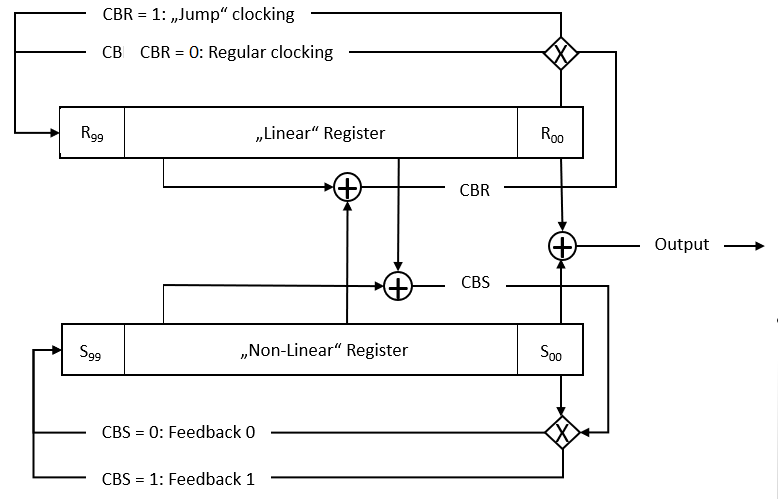
\includegraphics[width=1\textwidth]{img/mickeyv2.png} 
				\caption{Internal structure of the MICKEY v2 ciphe}
				\label{fig:mickeyv2}
			\end{subfigure}
			\begin{subfigure}{0.5\textwidth}
				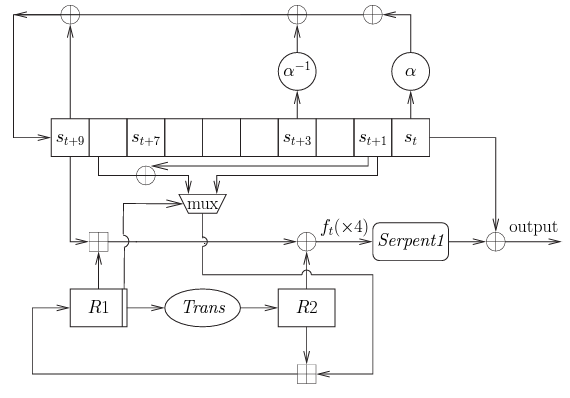
\includegraphics[width=1\textwidth]{img/SOSEMANUK.png} 
				\caption{Internal structure of the SOSEMANUK cipher}
				\label{fig:sosemanuk}
			\end{subfigure}
			
			\caption{LFSR-based eStream finalists}
			\label{fig:lfsr}
			
		\end{figure}
		
		
		\emph{Mickey v2} is a bit-oriented LFSR-based cipher. It uses irregular timing of shift registers, as well as new methods that provide a sufficiently large period and pseudo-randomness of the key sequence and resistance to attacks \cite{babbage2006stream}. As of 2013, a differential fault attack has been reported \cite{banik2015improved}.\\
		\emph{SOSEMANUK} is a word-oriented LFSR-based cipher influenced by the stream cipher SNOW and the block cipher SERPENT. Like the SNOW cipher, the SOSEMANUK algorithm uses two basic concepts: an LFSR and an FSM. The data obtained using the LFSR is fed to the input of the FSM, where it is non-linearly transformed. The four output values of the state machine are then table-swapped and XORed with the appropriate shift register values. The key schedule for the cipher is compiled using the Serpent24 primitive \cite{berbain2008sosemanuk}. Several attacks on SOSEMANUK have been published \cite{tsunoo2006evaluation} \cite{lee2008cryptanalysis}. However, none of the proposed attacks breaks the claimed 128-bit security of the cipher.
		
		\item [Random shuffled] stream ciphers achieve high efficiency of software implementation by employing randomly shuffled tables that shuffle a list to create random permutations, based on the RC4 cipher design. Since RC4 has got a number of applications in practice, it inspired subsequent designs of this type of structure, against which the state recovery attacks often require extremely high time complexity \cite{jiao2020stream}. 
		
		\begin{figure}[h]
			\centering
			\includegraphics[width=.5\textwidth]{img/hc-128.png}
			\caption{Internal structure of the HC-128 random shuffled cipher}
		\end{figure}
		
		A representative of this category in the eStream portfolio is the \emph{HC-128} cipher. Its internal state consists of two tables, each with 512 registers of 32 bits in length. At each step, one register of one of the tables is updated using a non-linear feedback function, while one 32-bit output is generated from the non-linear output filtering function. The cipher specifications state that 264 bits can be generated from each key/IV pair \cite{wu2008stream}.
		Despite the design's high profile, there have been no significant cryptanalytic advances against HC-128 since the publication of the eSTREAM portfolio.
		
	\end{description}
	
	\section{Trivium}
	
	In this section, we would like to show the functionality of a stream cipher on the example of the Trivium. This cipher was chosen for two reasons:
	\begin{enumerate}
		\setlength\itemsep{0.1em}
		\item Trivium has a very simple design, perfect for illustrative purposes.
		\item Trivium scored very highly at the SASC 2008 evaluation.
	\end{enumerate}
	
	\subsection{Functionality}
	
	Trivium consists of the following phases \cite{canniere2008trivium}:
	\begin{enumerate}
		\item \textbf{Initialization}
		\begin{itemize}
			\setlength\itemsep{0.1em}
			\item[-] IV: 80 bits.
			\item[-] Key: 80 bits.
			\item[-] Internal state: 288 bits ($s_1$, . . . , $s_{288}$). 
			\item[-] 4 * 288 = 1152 randomization cycles (after 1152 cycles a key stream is generated).
			\item[-] Key stream: N $\leq$ $2^{64}$ ($z_0$, ..., $z_n$), where N is the length of the plaintext.
		\end{itemize}
		At first, the  80-bit key (K) and an 80-bit initialization vector (IV) are loaded into the 288-bit internal state, all the remaining bits are set to 0s, except the last three, which are set to 1s. Then the bits in the register are randomized and rotated over 4 full cycles without generating keystream bits to improve randomization as well as dependency between the internal state, key and the initialization vector .
		The pseudo-code below shows the process in more detail:
		\vspace{0.5em}
		\\
		{\fontfamily{qcr}\selectfont
			($s_1$, $s_2$, ..., $s_93$) ← ($K_1$, ..., $K_{80}$, 0, ..., 0)\\
			($s_{94}$, $s_{95}$, ..., $s_{177}$) ← ($IV_1$, ..., $IV_{80}$, 0, ..., 0)\\
			($s_{178}$, $s_{279}$, ..., $s_{288}$) ← (0, ..., 0, 1, 1, 1)\\
			\textbf{for} i = 1 to 4 * 288 \textbf{do} \\
			\indent\hspace{1cm}$t_1$ ← $s_{66}$ $\oplus$ $s_{91}$ $\odot$ $s_{92}$ $\oplus$ $s_{93}$ $\oplus$ $s_{171}$\\
			\indent\hspace{1cm} $t_2$ ← $s_{162}$ $\oplus$ $s_{175}$ $\odot$ $s_{176}$ $\oplus$ $s_{177}$ $\oplus$ $s_{264}$\\
			\indent\hspace{1cm} $t_3$ ← $s_{243}$ $\oplus$ $s_{286}$ $\odot$ $s_{287}$ $\oplus$ $s_{288}$ $\oplus$ $s_{69}$\\
			\indent\hspace{1cm}($s_1$, $s_2$, ..., $s_{93}$) ← ($t_3$, $s_1$, ..., $s_{92}$)\\
			\indent\hspace{1cm}($s_{94}$, $s_{95}$, ..., $s_{177}$) ← ($t_1$, $s_{94}$, ..., $s_{176}$)\\
			\indent\hspace{1cm}($s_{178}$, $s_{279}$, ..., $s_{288}$) ← ($t_2$, $s_{178}$, ..., $s_{287}$)\\
			\textbf{end for}\\
		}
		\\
		The initialization procedure ensures that every bit of the initial state depends on every bit of the key and every bit of the initialization vector. This effect is achieved already after 2 full cycles (2*288 cycle executions). 2 more cycles are needed to complicate the bit relationships. For example, the first 128 bytes of the keystream, obtained from the null key and the initialization vector, have approximately the same number of 1s and 0s evenly distributed. Even with the simplest and identical keys, the Trivium algorithm produces a sequence of numbers that is close to random.
		\item \textbf{Stream generation}
		
		The keystream generation consists of an iterative process that extracts the values of 15 specific state bits and uses them both to update 3 bits of the state and to compute 1 bit of keystream $z_i$. The state bits are then rotated and the
		the process repeats itself until the requested N $\leq$ $2^{64}$ bits of keystream have been generated. The following pseudo-code describes the process in more detail:
		\vspace{0.5em}
		\\
		{\fontfamily{qcr}\selectfont
			\textbf{for} i = 1 \textbf{to} N \textbf{do}\\
			\indent\hspace{1cm}$t_1$ ← $s_{66}$ $\oplus$ $s_{93}$\\
			\indent\hspace{1cm}$t_2$ ← $s_{162}$ $\oplus$ $s_{177}$\\
			\indent\hspace{1cm}$t_3$ ← $s_{243}$ $\oplus$ $s_{288}$\\
			\indent\hspace{1cm}$z_i$ ← $t_1$ $\oplus$ $t_2$ $\oplus$ $t_3$\\
			\indent\hspace{1cm}$t_1$ ← $t_1$ $\oplus$ $s_{91}$ $\odot$ $s_{92}$ $\oplus$ $s_{171}$\\
			\indent\hspace{1cm}$t_2$ ← $t_2$ $\oplus$ $s_{175}$ $\odot$ $s_{176}$ $\oplus$ $s_{264}$\\
			\indent\hspace{1cm}$t_3$ ← $t_3$ $\oplus$ $s_{286}$ $\odot$ $s_{287}$ $\oplus$ $s_{69}$\\
			\indent\hspace{1cm}($s_1$, $s_2$, ..., $s_{93}$) ← ($t_3$, $s_1$, ..., $s_{92}$)\\
			\indent\hspace{1cm}($s_{94}$, $s_{95}$, ..., $s_{177}$) ← ($t_1$, $s_{94}$, ..., $s_{176}$)\\
			\indent\hspace{1cm}($s_{178}$, $s_{279}$, ..., $s_{288}$) ← ($t_2$, $s_{178}$, ..., $s_{287}$)\\
			\textbf{end for}
		}
	\end{enumerate}
	
	To better understand the algorithm, consider this example:
	\begin{enumerate}
		\setlength\itemsep{0.1em}
		\item We initialize a plaintext. For simplicity, it we will take an 'a'.\\
		{\fontfamily{qcr}\selectfont
			plainText = 0110 0001
		}
		
		
		\item We initialize a random initialization vector (IV) and a random key (K), 80 bits each.\\
		{\fontfamily{qcr}\selectfont
			\emph{K} = 0010 0101 1001 0101 1010 1011 0000 0011 0000 1101 0011\\
			\indent\hspace{1cm}1100 0010 0100 0001 0001 0111 0110 1110 1010
		}
		\vspace{0.5em}
		\\
		{\fontfamily{qcr}\selectfont
			\emph{IV} = 0111 0000 1100 0001 0101 0111 1100 0110 1101 0111 1110\\ 
			\indent\hspace{1.2cm}1000 1011 0111 0001 0000 1110 1110 0000 0111
		}
		
		\item For this example we initialize three shift registers, 288 bits in total. Where \emph{regA} is 93 bits long, \emph{regB} - 84 bits, and \emph{regC} is 111 bits long. The registers have to be loaded with the \emph{IV} and the \emph{K}. \\
		The first 80 bits of \emph{regA} are loaded with the \emph{K}, and the rest are 0. 
		\vspace{0.5em}
		\\
		{\fontfamily{qcr}\selectfont
			\emph{regA} = 0010 0101 1001 0101 1010 1011 0000 0011 0000 1101 0011 \\ 
			\indent\hspace{1.6cm}1100 0010 0100 0001 0001 0111 \textbf{0}110 1110 1\textbf{0}10 0\textbf{000}  0000\\
			\indent\hspace{1.6cm}00\textbf{00} \textbf{0}
		}
		\vspace{0.5em}
		\\
		The first 80 bits of \emph{regB} are loaded with \emph{IV}, the rest is 0. \\
		{\fontfamily{qcr}\selectfont
			\emph{regB} = 0111 0000 1100 0001 0101 0111 1100 0110 1101 0111 1110 \\ 
			\indent\hspace{1.6cm}1000 1011 0111 0001 0000 1\textbf{1}10 \textbf{1}110 0000 0111 0\textbf{000}
		}
		
		The last three bits of \emph{regC} are 1, the rest are 0.
		\vspace{0.5em}
		\\
		{\fontfamily{qcr}\selectfont
			\emph{regC} = 0000 0000 0000 0000 0000 0000 0000 0000 0000 0000 0000 \\ 
			\indent\hspace{1.6cm}1000 0000 0000 0000 0000 0\textbf{0}00 0000 0000 0000 0000 00\textbf{0}0 \\ 
			\indent\hspace{1.6cm}0000 0000 0000 0000 0000 \textbf{111}
		}
		\item As it is shown in the pseudo-code above, the bits are randomized with the help of XOR and AND operations, applied to the state register bits at the positions: 
		\vspace{0.5em}
		\\
		$regA_{66}$, $regA_{69}$, $regA_{91}$, $regA_{92}$, $regA_{93}$, \\
		$regB_{69}$, $regB_{78}$, $regB_{82}$, $regB_{83}$, $regB_{84}$, \\
		$regC_{66}$, $regC_{87}$, $regC_{109}$, $regC_{110}$, $regC_{111}$.
		\vspace{0.5em}
		\\
		This is repeated for four cycles.\\
		Operations with these chosen bits guarantee the longest period before bits start to repeat.\\
		After the randomization we get the following:
		
		{\fontfamily{qcr}\selectfont
			
			\emph{regA} = 1101 0111 1001 1001 0110 0111 0001 0010 1010 1000 0101 \\ 
			\indent\hspace{1.6cm}1000 1010 1011 1111 1100 0\textbf{1}10 \textbf{1}011 1001 0110 1100 1110 \\ 
			\indent\hspace{1.6cm}01\textbf{00} \textbf{1}
			
			\emph{regB} = 1101 1101 1101 0101 0111 0101 0011 1110 0001 0101 0011 \\ 
			\indent\hspace{1.6cm}1000 0011 0001 0111 0111 0011 \textbf{0}011 1001 1\textbf{1}10 1\textbf{100}
			
			\emph{regC} = 1111 0011 0000 0111 1001 0110 0101 0001 0100 0010 1011 \\ 
			\indent\hspace{1.6cm}1100 0000 0000 0011 1110 0\textbf{1}10 0001 1010 \textbf{1}000 1101 0111 \\
			\indent\hspace{1.6cm}0011 1010 1001 1000 100\textbf{0} \textbf{01}
		}
		\item Next step is the key generation. The procedure is similar to the Key and IV initialization, but now a key stream, the same length as the \emph{plainText}, is generated from the output variables:\\
		{\fontfamily{qcr}\selectfont
			$z_i$ ← $t_1$ $\oplus$ $t_2$ $\oplus$ $t_3$\\
			Where \\
			$t_1$ = $regA_{66}$ $\oplus$ $regA_{93}$\\
			$t_2$ = $regB_{69}$ $\oplus$ $regB_{84}$\\
			$t_3$ = $regC_{66}$ $\oplus$ $regC{111}$
		}
		\item \emph{$t_3$}, \emph{$t_1$}, \emph{$t_2$} are then added in the beginning of the \emph{regA}, \emph{regB}, \emph{regC} respectively, shifting this way bites. After eight iterations we have our \emph{keyStream}:\\
		{\fontfamily{qcr}\selectfont
			keyStream  = z = 0101 0111 = 'W'
		}
		\item Finally an encrypted text is generated by XORing corresponding bits from the key stream and from the plainText.\\
		{\fontfamily{qcr}\selectfont
			encryptedText = 0101 0111 $\oplus$ 0110 0001 = 0011 0110 = 6
		}
		\item By XORing the encrypted text with a keyStream, we can get our plain text back.\\
		{\fontfamily{qcr}\selectfont
			plainText = 0011 0110 $\oplus$ 0101 0111 = 0110 0001 = 'a'
		}
	\end{enumerate}
	
	\subsection{Security}
	According to the authors of the cipher \cite{canniere2008trivium}, it is harder to find \emph{correlations} between the internal state bits and the keystream in Trivium because as opposed to LFSR based ciphers, Trivium's state register is updated in a non-linear way, so it is harder for an attacker to recover the state.\\
	The non-linear nature of the cipher makes it nearly immune to the attacks that rely on determining its \emph{period} as well as \emph{algebraic attacks}. \emph{Resynchronization attacks} are avoided by cycling the state four times (step 4 in the example above) before producing any output. The authors name \emph{Guess and Determine attacks} as the ones of the most concern.\\
	In 2013 another team of researchers has shown that Trivium can be broken by a \emph{cube attack}, if the number of initialization rounds is reduced to 799 \cite{fouque2013improving}. 
	Only in 2020 \cite{potestad2020breaking} a not reduced version of Trivium was broken with the help of \emph{Experimental Attacks and Differential fault analysis (DFA)}. The idea is to inject faults into the Trivium clock cycle and get the faulty outputs. Then with the help of DFA the internal state is recovered through a comparison between correct and faulty outputs, after that, a specially designed Trivium version goes back and gets the initial key and the internal state. According to the authors, 100\% of keys have been recovered using this method.
	
	\section{Conclusion}
	In this paper, we have shown the principles, functionality, and mathematical basis of stream ciphers as well as evaluated their security. It is easy to notice that stream ciphers are a huge family united by the idea of streams of random numbers. And continuing the thought of John von Neumann, "...no such thing as a random number - there are only methods to produce random numbers." \cite[p.~36]{vonNeumann1951} we see that the variety of stream cipher designs is built on a pseudo-random flow of digits, which is just good enough to make things difficult for an attacker. Although all stream ciphers have an LFSR in them, it would be very insecure to use only an LFSR to create a random digit stream. LFSRs are not cryptographically secure because they are easy to reverse engineer. That is why stream ciphers usually have a non-linear part to improve security.\\
	As a result of our research, the following advantages of stream ciphers over block ciphers can be defined:
	\begin{enumerate}
		\setlength\itemsep{0.1em}
		\item Due to bit-by-bit operations, stream ciphers are more efficient and faster than block ciphers.
		\item They are better suited for environments with limited resources. 
		\item If there’s an error in one symbol, it’ll be less likely to affect the next.
		\item Easy to implement in hardware, using Flip-Flops and gates.
	\end{enumerate}
	The main disadvantages of stream ciphers, however, are:
	\begin{enumerate}
		\setlength\itemsep{0.1em}
		\item Due to looping in LFSRs, stream ciphers are not very software efficient.
		\item Stream ciphers are very vulnerable to bit-flipping and code reuse attacks because of their bit-by-bit approach. 
		\item Because stream ciphers work not with blocks, but with bits, an adversary can change a strategically chosen bit in the encrypted text to change the decrypted one.
	\end{enumerate}
	
	Stream ciphers are usually used where the amount of data is unknown or may be continuous, for example in wireless networking, or in the military. Nowadays the most common stream cipher used is ChaCha, which is based on Salsa20 we mentioned earlier, and its variations. \\
	Although stream ciphers are not especially widely used, it has been shown that they have their own niche, where they have considerable advantages over block ciphers and therefore more research should be put into this type of ciphers.
	\clearpage

\pagebreak

\listoffigures

\pagebreak

\printbibliography %Citavi 5

\end{document}
